%!TEX root = ./main.tex

\section{Experiments}

\paragraph{Setting.}
To evaluate the empirical performance of our proposed algorithm, we conducted experiments on routing problems
that are motivated by congestion management.
In the routing problem, we are given a directed graph $G(A,V)$, a set of requests $R = \{(s_{i}, t_{i}) : s_{i}, t_{i} \in V\}$ that represents demands of
connecting $s_{i}$ to $t_{i}$. We assume that for each request, there exists a directed path between $s_{i}$ to $t_{i}$.
Each arc $(u, v) \in A$ is associated with a cost function $f_{(u,v)}: \mathbb{R}^{+} \rightarrow \mathbb{R}^{+}$ that depends on the number of requests using the arc.
Requests arrive online, and the goal is to design a routing that minimizes the total cost.


\paragraph{Input.}
There are two type of inputs in our experiments. The first one includes randomly generated graphs following the Erd\H{o}s-Rényi model $G(n, p)$, where $n$ is the number of vertices and $p$ is the probability that an arc gets created. The source and target vertices of the requests are also generated uniformly at random. The second input type collects specific examples designed to trap algorithms which rely on greedy heuristics.


\paragraph{Predictions.}
The predictions come from rounding the optimal offline fractional solution. If a request is served by several paths in the fractional solution, the oracle picks one of the paths uniformly at random using the amounts passing through each of them as weights. Otherwise, the oracle uses the unique best path of the optimal solution. Due to the randomized rounding, on most instances the oracles propose a worse solution than the optimal greedy integral solution, which picks the cheapest path at each time step.


\paragraph{Implementation.}
The routing problem's covering formulation enumerates all possible cuts in the graph. Upon each arriving request $r = (s,t)$, a new set of constraints are released $\sum_{e \in \delta(S)} x_{e}^{r} \ge 1$, where $\delta(S)$ is the cut on $S \subset V$ such that $s \in S$ and $t \notin S$. This formulation generates an exponential number of constraints with respect to the size of the graph. However, these constraints can be simplified in the implementation of Algorithm~\ref{algo:covering}, since the algorithm is not constrained by standard linear program solving techniques. Algorithm~\ref{algo:covering} increases the amount of traffic on each arc following the step described on line \ref{algo-covering:x}. The request is satisfied when there exists a path among the arcs in the set $A^{*}$ (arcs with value $1$). Therefore, we can replace the constraint satisfaction with a simple path finding in the implementation. If there are several possible paths with the arcs in $A^{*}$, our algorithm chooses the minimum cost path, so the implementation includes a rounding step providing an integral solution.


\paragraph{Instances.} Randomly generated instances yield similar results, therefore we only present one of them, named Instance $1$. Additionally, we show an example, where the greedy heuristic makes sub-optimal decisions on Instance $2$. These two instances are complementary and allow us to examine how our algorithm behaves when the oracles' predictions are worse or better than the greedy heuristic.

\textit{Instance $1$} has $20$ vertices, $184$ arcs, and $20$ requests. Each arc has a cost function of the form $f(x) = a x^b$, where $1.0 \le a \le 10.0$ and $1.0 \le b \le 4.0$. We generated $20$ oracles from the optimal offline fractional solution and kept $3$ of these oracles: the best, the worst and the middle one on the scale of their obtained objective values.

\textit{Instance $2$} has $8$ vertices, $16$ arcs, and $7$ requests. This instance is specifically designed to trap the greedy heuristic. The structure of Instance $2$ is visible on ??? Figure, along with the greedy and optimal solutions.

\paragraph{Observation.} When the prediction is not an optimal offline solution (the error is not 0),
our algorithm outperforms both the prediction and the greedy solution when the confidence parameter is $0.1 \leq \eta \leq 0.8$.
In practice, predictions are neither perfect nor completely wrong. So the confidence parameter, reflecting the reliability of the predictions,
is rarely very close to 0 nor very close to 1. The experiments prove that our algorithm provides improvements over the predictions and the greedy solution
(achieving the best theoretical performance) in the practical aspect of the routing problem.

{
    \begin{minipage}{0.3\textwidth}
        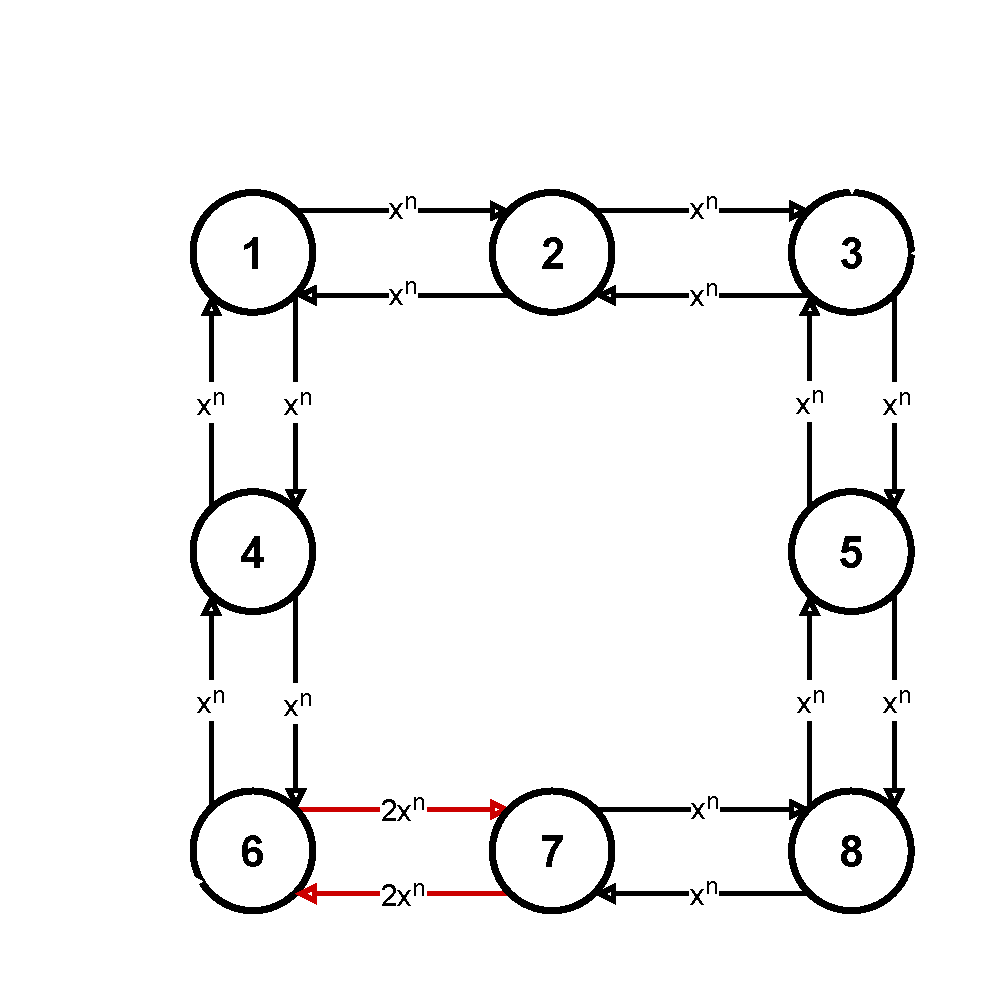
\includegraphics[width=\linewidth]{Img/cex_init2.pdf}
    \end{minipage}
    \begin{minipage}{0.3\textwidth}
        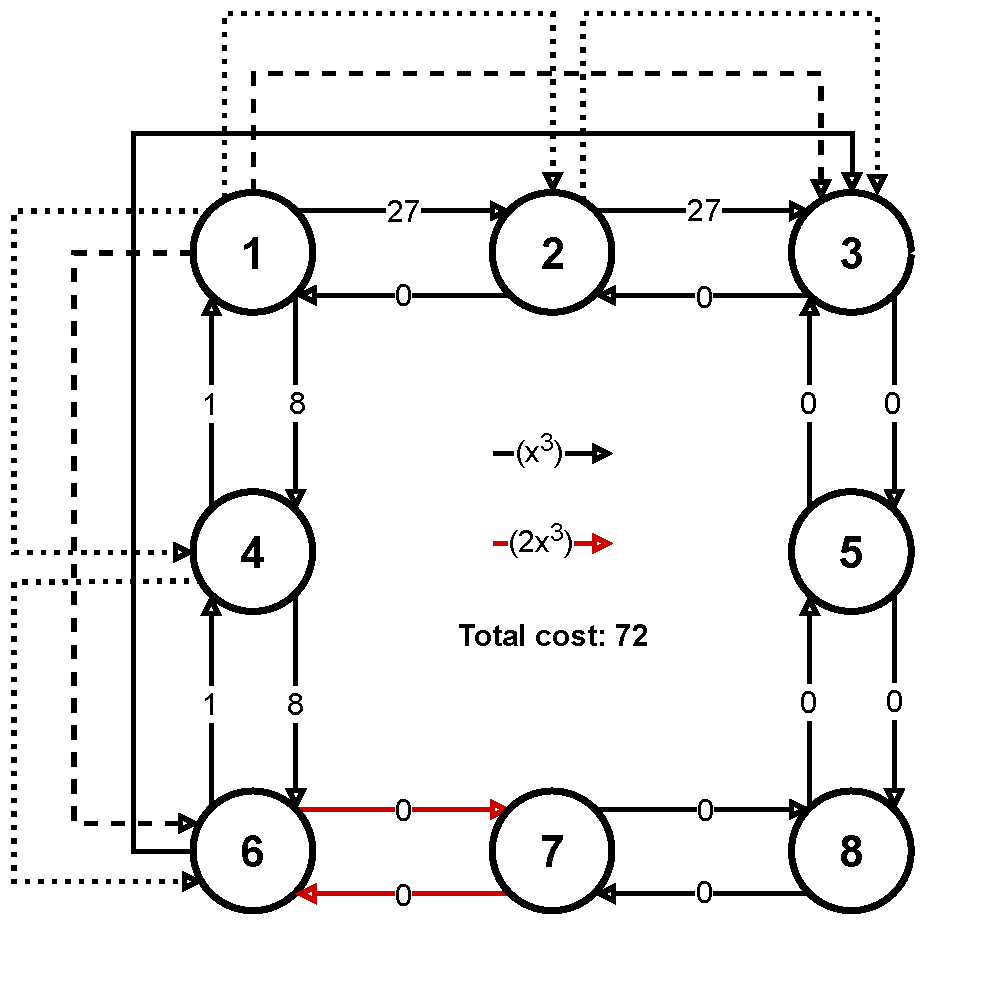
\includegraphics[width=\linewidth]{Img/cex_greedy2.pdf}
    \end{minipage}
    \begin{minipage}{0.3\textwidth}
        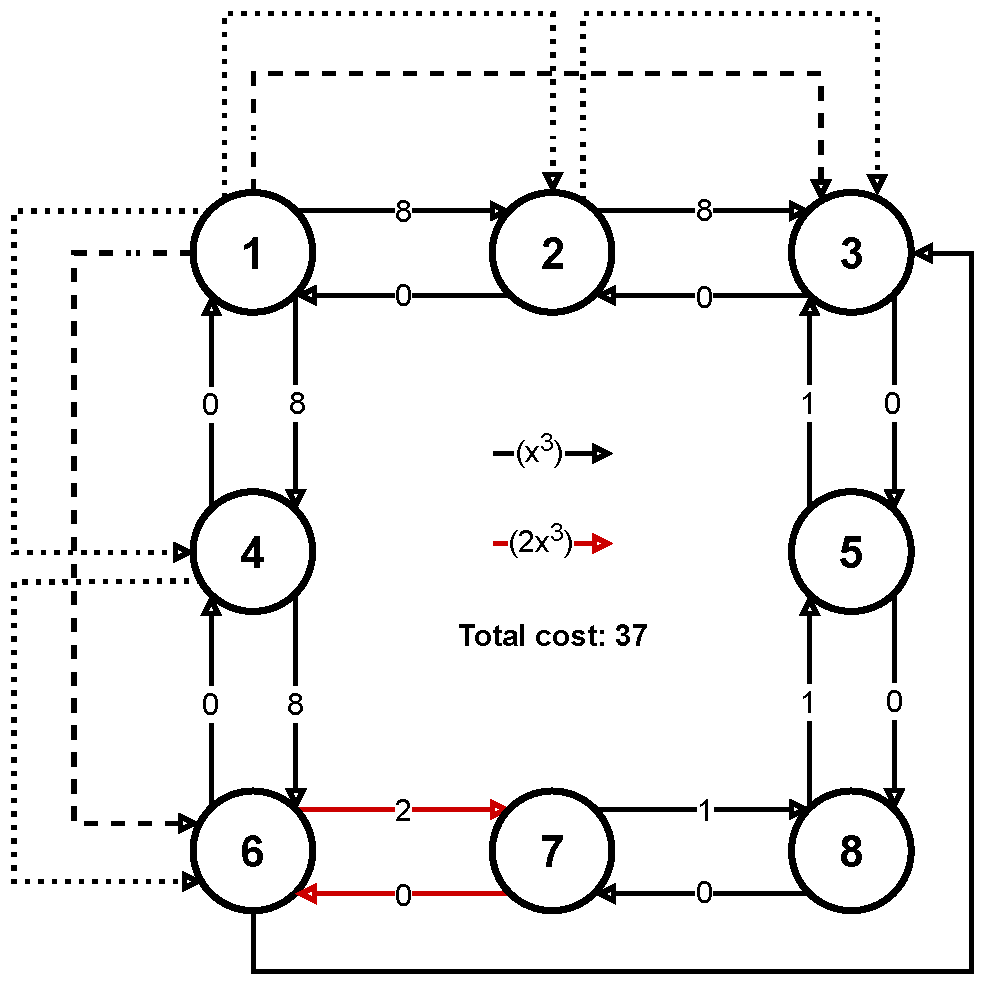
\includegraphics[width=\linewidth]{Img/cex_opt2.pdf}
    \end{minipage}
    \captionof{figure}{Instance $2$, the greedy solution, and the optimal solution}
    \label{fig:cex}
}
